%\clearpage
%\clearpage
%\input{../introduction/problem.tex}
%%\clearpage
%\input{../introduction/goal.tex}
%%\clearpage
%\input{../introduction/mission.tex}
\section{Introduction}
Following all disturbances such as air resistance are neglected. Also, the rocket can be below the y axis. Although it is assumed that this is mostly the ground.\\
Here is the timeline of the flight:

	\begin{enumerate}
		\item \textbf{Propelled up time} 0.15 seconds with 16N
		\item \textbf{Parabel flight} Until the parachute ist open at a velocity of $-20^m/_s$
		\item \textbf{Parachute flight} Constant velocity of $-20^m/_s$
	\end{enumerate}
Here are equations for the model:
	\begin{eqnarray}
		v\left( t\right)  &=& v_0 + a * t\\
		x\left( t\right)  &=& x_0 + v_0 * t + 0.5 * a * t^2\\
		x &=& \int \dot{x_0}  dt + \iint \ddot{x}  dt^2 + x_0
	\end{eqnarray}
	
	
	
	
\section{Model}\label{sec:model}
The variables were imported from the Matlab script in the handout. The code is also in this documentation in Listing \ref{lst:code1}.
The sign of g was changed to minus. Because the coordinate system is oriented upwards.
With the variables and equations from the handout, a Simulink model was built shown in Figure \ref{fig:overview}.
The input of the model is the acceleration. This is integrated first to the speed and then to the height. All three signals are visualized with the scope.
	


	\begin{figure}[H]
		\centering
		\includegraphics[width=0.7\textwidth]{figures/overview.png}
		\caption{Overview of the simulink model.}
		\label{fig:overview}
	\end{figure}

	

	\subsection{Propelled up}
	In the first 0.15s the rocket is propelled up by a force of 16N. The acceleration from the rocket is calculated in Equation \ref{eq:acc}. The gravity is there subtracted too.
		\begin{equation}
			a_{Rocket} = \frac{F}{m} + g = \frac{16N}{0.05kg} - 9.81^m/_{s^2} = 310^m/_{s^2} \label{eq:acc}
		\end{equation}
	The velocity increases rapidly in a linear manner. The height becomes larger quadratically. This can be seen in Figure \ref{fig:overview}. The force is symbolized by the step on the right hand side. The force is divided by the mass m and then g is added to it.
	
	
	\subsection{Paraple flight}
	After this 0.15s the only force that still affects the rocket is the gravity with the known $-9.81^m/_{s^2}$. 
	The velocity becomes linearly smaller and after it breaks the zero line it becomes linearly larger in the negative. 
	The height makes a parable. After the slope first decreases, it becomes negative after the velocity is negative.
	
	
	\subsection{Parachute flight}
	When the negative velocity is higher then $20^m/_s$ the parachute opens and the velosity stays constant by $-20^m/_s$. That means the acceleration is zero. This is solved in the model as follows. When the velocity is smaller then vChute the output from the comperator is one. This is gained with g and and subtracted from the general acceleration.
	


\section{Simulation}
The process described in Section \ref{sec:model} can be shown in Figure \ref{fig:scope1}. 
The graph on the top is the hight in meter and the parable flight is good visible in contrast to the changes. 
The graph in the middle is the velocity in meter per second. Here, all changes are easily recognizable and also that the velocity get negative.
The graph on the bottom is the acceleration.The propelled up in the first 0.15 seconds is good visible and also the change after this part. The change from the paraple flight to the parachute flight is not recognizable at the first glance. It is the small step at about seven seconds.
	
	
	\begin{figure}[H]
		\centering
		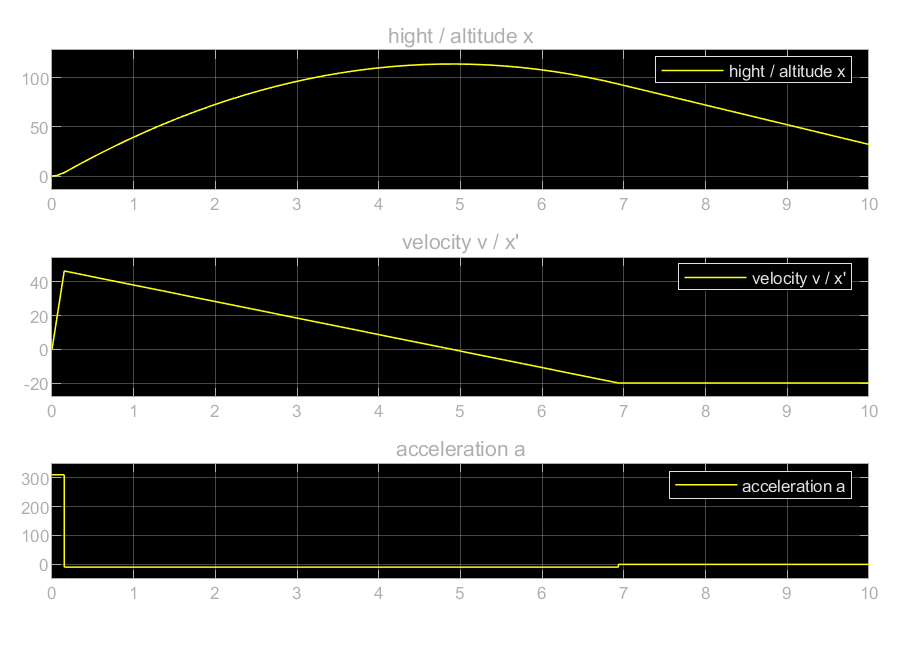
\includegraphics[width=0.7\textwidth]{figures/scope.eps}
		\caption{Scope from the Simulation.}
		\label{fig:scope1}
	\end{figure}

\newpage

\section{Code Analysis}
The code is in Listing \ref{lst:code1}
At the top is the variable declaration and the reset of the running variables.
Then the code is divided into three loops. These are the parts of the flight, the propelled up, the paraple flight and the parachute flight. The position of the rocket is calculated with the forward euler.\\
The stepsize is set with Dt and n is a controlvariable. If n > 50000 all loops break and the script runs to the end. One case is when Dt is to small.\\
On Figure \ref{fig:plot1} is the visualisation of velocity and position. the red '+' is when the propelled up turns off and the red 'o' is when the parachute opens.

	\begin{figure}[H]
		\centering
		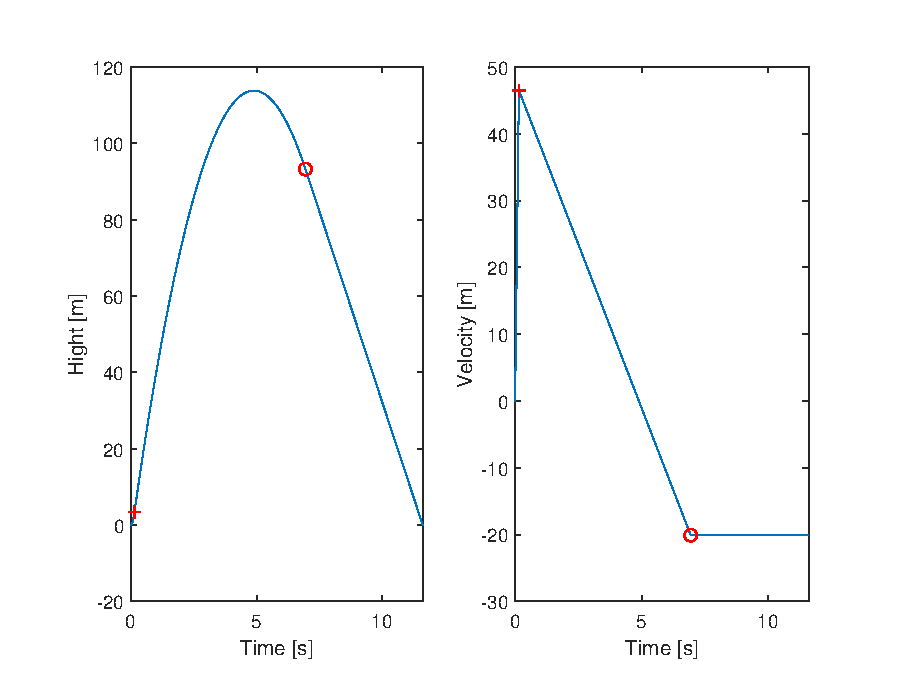
\includegraphics[width=0.7\textwidth]{figures/plot1.eps}
		\caption{Plot from running code in Listing \ref{lst:code1}.}
		\label{fig:plot1}
	\end{figure}
	
\newpage
\begin{lstlisting}[caption={Matlabcode from the handout},label=lst:code1]
	clear all; clc; close all;	
	%%
	% g inverted
	m=0.05; g=-9.81; tEngine=0.15; Force=16; vChute=-20; Dt=0.01; 
	clear t v h 
	n=1; 
	t(n)=0; v(n)=0; h(n)=0; t(2)=0;
	
	%%
	% Segment 1 
	a1=(Force+m*g)/m; 
	while (t(n) < tEngine) &&  (n < 50000) 
	n=n+1; 
	t(n)=t(n-1)+Dt; 
	v(n) =a1 *t (n) ; 
	h(n) =0.5*a1*t(n)^2;
	end;
	v1=v(n); h1=h(n); t1=t(n);
	
	% Segment 2
	while v(n)>=vChute && n<50000
	n=n+1;
	t(n)=t(n-1)+Dt;
	v(n)=v1+g*(t(n)-t1);
	h(n) =h1+v1 * (t(n)-t1 )+0.5*g* (t (n)-t1)^2;
	end
	v2=v(n); h2=h(n); t2=t(n);
	
	% Segment 3
	while h(n)>0 && n<50000
	n=n+1;
	t(n)=t(n-1)+Dt;
	v(n)=vChute;
	h (n) =h2+vChute* (t(n)-t2) ;
	end
	
	%%
	subplot(1,2,1)
	plot(t,h,t2,h2, 'ro', t1, h1, 'r+')
	xlabel('Time [s]');
	ylabel('Hight [m]');
	subplot(1,2,2)
	plot(t,v,t2,v2, 'ro', t1, v1, 'r+')
	xlabel('Time [s]');
	ylabel('Velocity [m]');
	
	
	%%
	% Analysis of the loged datas. 
	a = logsout{1}.Values.Data;
	v = logsout{2}.Values.Data;
	x = logsout{3}.Values.Data;
	t_log = logsout{2}.Values.Time;
\end{lstlisting}
	
	
\section{Conclusion}
